\subsubsection{Scattering of Scalar Nucleons}
Let's go back to the scalar Yukawa theory of the section \ref{sec:ScYukawa} and 
consider nucleon scattering process $\psi \psi \to \psi \psi$.
\begin{eqnarray}
\begin{array}{l}
\ketend i \ket
=
b^\dagger(\bld{p}_a) b^\dagger(\bld{p}_b) \ketend 0 \ket
\rightdef
\ketend N_a N_b \ket
\\
\ketend f \ket
=
b^\dagger(\bld{p}_1) b^\dagger(\bld{p}_2) \ketend 0 \ket
\rightdef
\ketend N_1 N_2 \ket
\end{array}
\end{eqnarray}
The first contribution to $S - 1$ in Eq. (\ref{eqn:SmatrixPertSerCov}) arise from 
the term of the second order in ${\cal H}_{int}$. It reads
\begin{eqnarray}
\bra f \braend S^{(2)} \ketend i \ket
&=&
\frac{(-i g)^2}{2} \int d^4 x_1 d^4 x_2
\bra f \braend
T[
\normalprod{\psi^\dagger(x_1) \psi(x_1) \phi(x_1)}
\nonumber\\
&&
\hspace{35mm}
\times
\normalprod{\psi^\dagger(x_2) \psi(x_2) \phi(x_2)}
]
\ketend i \ket
\nonumber\\
&=&
\frac{(-i g)^2}{2} \int d^4 x_1 d^4 x_2
\Delta_F(x_1 - x_2)
\nonumber\\
&&
\hspace{12mm}
\bra N_2 N_1 \braend
\normalprod{
\psi^\dagger(x_1) \psi(x_1) 
\psi^\dagger(x_2) \psi(x_2)
}
\ketend N_a N_b \ket\,,
\nonumber\\
\label{eqn:scYS2ndord}
\end{eqnarray}
%-------------------------------------------
The sandwich $\bra N_1 N_2 \braend \dots \ketend N_b N_a \ket$ reads
\begin{eqnarray}
&&\bra N_1 N_2 \braend
\normalprod{
\psi^\dagger(x_1) \psi(x_1) 
\psi^\dagger(x_2) \psi(x_2)
}
\ketend N_b N_a \ket
\nonumber\\
&=&
\int \frac{d^3 \bld{p}_1' d^3 \bld{p}_2'}{(2\pi)^3 4 {p_1^0}' {p_2^0}'} 
 \frac{d^3 \bld{p}_a' d^3 \bld{p}_b'}{(2\pi)^3 4 {p_a^0}' {p_b^0}'} 
 e^{i(p_1' x_1 + p_2' x_2 - p_a' x_1 - p_b' x_2)}
\nonumber\\
&&
 \bra 0 \braend 
 b(\bld{p}_2)  b(\bld{p}_1) \left\{
 b^\dagger(\bld{p}_1') b^\dagger(\bld{p}_2')
b(\bld{p}_a') b(\bld{p}_b')
\right\}
 b^\dagger(\bld{p}_a) b^\dagger(\bld{p}_b)
 \ketend 0 \ket
\nonumber\\
&=&
\int \frac{d^3 \bld{p}_1' d^3 \bld{p}_2'}{(2\pi)^3 4 {p_1^0}' {p_2^0}'} 
 \frac{d^3 \bld{p}_a' d^3 \bld{p}_b'}{(2\pi)^3 4 {p_a^0}' {p_b^0}'} 
 e^{i(p_1' x_1 + p_2' x_2 - p_a' x_1 - p_b' x_2)}
\nonumber\\
&&
\bra 0 \braend 
 b(\bld{p}_2)  \left\{
 2{p_1^0}' \delta^3(\bld{p}_1' - \bld{p}_1) 
 + b^\dagger({\bld{p}_1'}) b({\bld{p}_1})
 \right\}
 b^\dagger({\bld{p}_2'})
 \nonumber\\
 &&
  b(\bld{p}_a')   \left\{
 2{p_b^0}' \delta^3(\bld{p}_b' - \bld{p}_a) 
 + b^\dagger({\bld{p}_a}) b({\bld{p}_b'})
  \right\}
  b^\dagger({\bld{p}_b})
   \ketend 0 \ket
\nonumber\\
&=&
\int \frac{d^3 \bld{p}_1' d^3 \bld{p}_2'}{(2\pi)^3 4 {p_1^0}' {p_2^0}'} 
 \frac{d^3 \bld{p}_a' d^3 \bld{p}_b'}{(2\pi)^3 4 {p_a^0}' {p_b^0}'} 
 e^{i(p_1' x_1 + p_2' x_2 - p_a' x_1 - p_b' x_2)}
\nonumber\\
&&
\bra 0 \braend 
\left\{
4{p_1^0}' {p_2^0}' \delta^3(\bld{p}_1' - \bld{p}_1) \delta^3(\bld{p}_2' - \bld{p}_2) 
+
4{p_1^0}' {p_2^0}' \delta^3(\bld{p}_1' - \bld{p}_2) \delta^3(\bld{p}_2' - \bld{p}_1) 
\right\}
\nonumber\\
&&
\left\{
4{p_a^0}' {p_b^0}' \delta^3(\bld{p}_a' - \bld{p}_b) \delta^3(\bld{p}_b' - \bld{p}_a) 
+
4{p_a^0}' {p_b^0}' \delta^3(\bld{p}_a' - \bld{p}_a) \delta^3(\bld{p}_b' - \bld{p}_b) 
\right\}
\ketend 0 \ket
\nonumber\\
&=&
\frac{1}{(2\pi)^6}
\left\{
e^{i(p_1 x_1 + p_2 x_2)} + e^{i(p_2 x_1 + p_1 x_2)}
\right\}
\left\{
e^{-i(p_a x_1 + p_b x_2)} + e^{-i(p_b x_1 + p_a x_2)}
\right\}
\nonumber
\end{eqnarray}
Substituting this result in Eq. (\ref{eqn:scYS2ndord}) and 
adopting the expression (\ref{eqn:scFeynmanProp}),
we obtain
\begin{eqnarray}
\bra f \braend S^{(2)} \ketend i \ket
&=&
\frac{(-i g)^2}{2 (2\pi)^6} \int \frac{d^4 k}{(2\pi)^4} 
\frac{i}{k^2 - m^2 + i\epsilon}
\int d^4 x_1 d^4 x_2
\left\{
e^{i(p_1 + k - p_a)x_1}e^{i(p_2 - k - p_b)}
\right.
\nonumber\\
&&
+
e^{i(p_2 + k - p_a)x_1}e^{i(p_1 - k - p_b)}
+
e^{i(p_1 + k - p_b)x_1}e^{i(p_2 - k - p_1)}
\nonumber\\
&&
\left.
+
e^{i(p_2 + k - p_b)x_1}e^{i(p_1 - k - p_a)}
\right\}
\nonumber\\
&=&
\frac{i(-i g)^2}{(2\pi)^6} \int 
\frac{(2\pi)^4 d^4 k}{k^2 - m^2 + i\epsilon}
\left\{
\delta^4(p_1 + k - p_a)\delta^4(p_2 - k - p_b)
\right.
\nonumber\\
&&
\left.
\hspace{35mm}
+
\delta^4(p_2 + k - p_a)\delta^4(p_1 - k - p_b)
\right\}
\label{eqn:scYSelem}
\\
&=&
\frac{i(-i g)^2}{(2\pi)^6} 
\left\{
\frac{1}{(p_1 - p_a)^2 - m^2}
+
\frac{1}{(p_2 - p_a)^2 - m^2}
\right\}
\nonumber\\
&&
\times (2\pi)^4 \delta^4(p_1 + p_2 - p_a - p_b)
\nonumber\\
&=&
\nonumber\\
&&
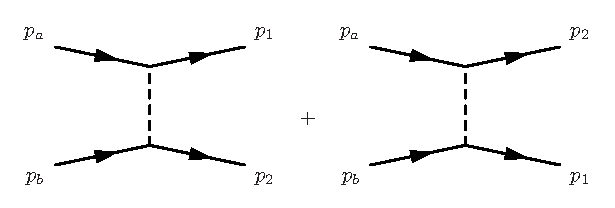
\includegraphics{\feynmfdirectory/01NNtoNNeq/NNtoNN.eps}
\nonumber\\
\label{eqn:scYSmtrxFeynmDiagNN}
\end{eqnarray}
%----------------------------------------
The final expression is written in terms of two Feynman diagrams
which correspond respectively to the two terms in Eq. (\ref{eqn:scYSelem}).
These diagrams are abbreviated a bit for a technical reason of the drawing.
A fully drawn diagram may look like the following figure.
\begin{figure}[h]
\vspace*{35mm}
%        positive in these values mean,  voffset: upward   hoffset: rightward
\special{psfile="\feynmfdirectory/02NNtoNNbig/NNtoNNtrim.eps" hscale=70 vscale=70 voffset=-0 hoffset=100}
\caption{Fully drawn Feynman diagram for the first term in Eq. (\ref{eqn:scYSmtrxFeynmDiagNN})}
\label{fig:scalarYNN2NNFeynm}
\end{figure}
Arrows on external lines indicate flows of conserved quantum numbers associated with
particles like baryon number, flavor and so on. In the present case, it is the electric charge
which is conserved in the Lagrangian density (\ref{eqn:sclYkwLagDens}) as is stated above
Eq. (\ref{eqn:scYelchrg}).
In many situations, we draw a diagram like Fig. \ref{fig:scalarYNN2NNFeynm} without
momentum arrows to represent the two diagrams in Eq. (\ref{eqn:scYSmtrxFeynmDiagNN}).


The correspondence between diagrams and equations are ensured by obeying
the so called Feynman rule described as follows:

\begin{enumerate}
\item For each external lines, associate a factor $1/\sqrt{(2\pi)^3}$.

\item To each vertex, associate a factor
\begin{eqnarray}
(-ig) (2\pi)^4 \delta^4(\sum_{in} p_{in})\,,
\end{eqnarray}
where $p_{in}$ denotes a momentum flowing into the vertex and the sum is taken
over all momenta connected to the vertex. Momenta flowing out from the vertex get
a minus sign. For the upper vertex in Fig. (\ref{fig:scalarYNN2NNFeynm}), for instance,
we read $\sum_{in} p_{in} = p_a - k - p_1$.

\item For each internal broken line, corresponding to a $\phi$ particle with momentum $k$,
write a factor of
\begin{eqnarray}
\int \frac{d^4 k}{(2\pi)^4} \frac{i}{k^2 - m^2 + i\epsilon}
\end{eqnarray}
When the internal line is solid, corresponding to a $\psi$ particle, write the same factor
with $m$ replaced by the nucleon mass $M$.
\end{enumerate}

The scattering amplitude $T_{fi} = \bra f \braend T \ketend i \ket$ 
in Eq. (\ref{eqn:Smatrix_and_T}) is now
written as
\begin{eqnarray}
T_{fi}^{(2)}
&=&
\frac{(-i g)^2}{(2\pi)^6} 
\left\{
\frac{1}{(p_1 - p_a)^2 - m^2}
+
\frac{1}{(p_2 - p_a)^2 - m^2}
\right\}
\nonumber\\
&=&
\frac{(-i g)^2}{(2\pi)^6} 
\left(
\frac{1}{t - m^2}
+
\frac{1}{u - m^2}
\right)
\end{eqnarray}
Finally, from Eq. (\ref{eqn:2to2cs}), we write the scattering cross section 
in scalar Yukawa theory to the lowest (second) order as
\begin{eqnarray}
\frac{d \sigma^{(2)}}{dt}
&=&
\frac{g^4}{16\pi \lambda(s, m_N^2,m_N^2)}
\left(
\frac{1}{t - m^2} + \frac{1}{u - m^2}
\right)^2
\label{eqn:scYNN2NNcs}
\end{eqnarray}

\bigskip

\noindent
\stepcounter{exercise}
Exercise\theexercise:
Examine the kinematical regions for $t$ and $u$ in this scattering.

\bigskip

An enhancement of the cross section at small $|t|$ follows from the mass pole
of the exchanged pion. We also understand an enhancement at small $|u|$ is
a consequence of  the domination of $t$-channel exchanges 
and the indistinguishability of the two nucleons in the final state.


%----------------------------------------
\begin{comment}
Integral expression of the scattering matrix element in Eq. (\ref{eqn:scYSelem}) 
is written in terms of the Feynman diagram as
\begin{figure}[h]
\vspace*{30mm}
%        positive in these values mean,  voffset: upward   hoffset: rightward
\special{psfile="\feynmfdirectory/01NNtoNNeq/NNtoNN.eps" hscale=70 vscale=70 voffset=30 hoffset=70}
%\caption{Feynman diagram}
\label{fig:scalarYNN2NNinEq}
\end{figure}


&&
\unitlength=1mm  %<<<---------------------------------------------- scale
\parbox{40mm}
{
\begin{fmffile}{NNbyPi1}
	\begin{fmfgraph*}(40,20)
			\fmfleft{i1,i2}
			\fmfright{o1,o2} 
			%\fmfv{label=$p_b$, label.angle=90}{i1}
			\fmflabel{$p_b$}{i1}
			\fmflabel{$p_a$}{i2}
			%\fmfv{label=$p_a$, label.angle=270}{i2}
			\fmflabel{$p_2$}{o1}
			\fmflabel{$p_1$}{o2}
			\fmf{fermion,tension=2}{i1,v1,o1}
			\fmf{fermion,tension=2}{i2,v2,o2}
			\fmf{dashes}{v1,v2}
			%\fmflabel{$-ig(2\pi)^4 \delta^4(\sum_{in} p_{in})$}{v1}
			%\fmflabel{$-ig(2\pi)^4 \delta^4(\sum_{in} p_{in})$}{v2}
	\end{fmfgraph*}
\end{fmffile}
}
\hspace{3mm}
+
\hspace{3mm}
\parbox{40mm}
{
\begin{fmffile}{NNbyPi2}
	\begin{fmfgraph*}(40,20)
			\fmfleft{i1,i2}
			\fmfright{o1,o2} 
			\fmflabel{$p_b$}{i1}
			\fmflabel{$p_a$}{i2}
			\fmflabel{$p_1$}{o1}
			\fmflabel{$p_2$}{o2}
			\fmf{fermion,tension=2}{i1,v1,o1}
			\fmf{fermion,tension=2}{i2,v2,o2}
			\fmf{dashes}{v1,v2}
	\end{fmfgraph*}
\end{fmffile}
}
\end{comment}
%----------------------------------------

\bigskip

\bigskip
%=================================================================
\noindent
\underline{$N\overline{N} \to N\overline{N}$ amplitude}

\bigskip

Initial and final states:
\begin{eqnarray}
\begin{array}{l}
\ketend i \ket
=
b^\dagger(\bld{p}_a) c^\dagger(\bld{p}_b) \ketend 0 \ket
\rightdef
%\ketend N(\bld{p}_a) \overline{N}(\bld{b}_b )\ket
\ketend N_a \overline{N}_b \ket
\\
\ketend f \ket
=
b^\dagger(\bld{p}_1) c^\dagger(\bld{p}_2) \ketend 0 \ket
\rightdef
%\ketend N(\bld{p}_1) \overline{N}(\bld{p}_2) \ket
\ketend N_1 \overline{N}_2 \ket
\end{array}
\label{eqn:scYNNbarNNbarinit}
\end{eqnarray}
Since there are four (anti) nucleons in the initial and final states, we need at least 
four $\psi$ (and $\psi^\dagger$) fields from interaction Hamiltonians and all $\phi$ fields should
be contracted out. Thus, S-matrix elements to the lowest order is written 
in the same form as Eq. (\ref{eqn:scYS2ndord}) with $N_b$ and $N_2$ replaced by
$\overline{N}_b$ and $\overline{N}_2$ respectively.
Evaluating the sandwich factor as before,
we get
\begin{eqnarray}
\bra f \braend S^{(2)} \ketend i \ket
%&\stackrel{(2)}{=}&
&=&
%\nonumber\\
%&&
\parbox{80mm}{
\includegraphics{\feynmfdirectory/03NNbar2NNbar/Smtrx2trim.eps}
}
\nonumber\\
\label{eqn:scYSmtrxFeynmDiagNNbar}
\end{eqnarray}
It reads
\begin{eqnarray}
T_{fi}^{(2)}
&=&
\frac{(-i g)^2}{(2\pi)^6} 
\left\{
\frac{1}{(p_a - p_1)^2 - m^2 \cancel{+ i\epsilon}}
+
\frac{1}{(p_a + p_b)^2 - m^2 + i\epsilon}
\right\}
\nonumber\\
&=&
\frac{(-i g)^2}{(2\pi)^6} 
\left(
\frac{1}{t - m^2}
+
\frac{1}{s - m^2 + i\epsilon}
\right)
\label{eqn:scYNNbar}
\end{eqnarray}
Cross section is obtained by adopting Eq. (\ref{eqn:2to2cs}) as before.
We omit $i \epsilon$ in the first term in Eq. (\ref{eqn:scYNNbar}) since
$t < 0$. In the second term, however, $s = m^2$ may occur when
$m > 2M$. This is why we remained $i \epsilon$ in the second term.
However, in this case, correction of the pion propagator due to higher
order terms with nucleon loops will bring a finite imaginary part into the
denominator of the propagator. Nevertheless, for the lowest order
tree diagram, we keep the $i \epsilon$ term. 

\bigskip

\verb/-----------.-----------.-----------.-----------.-----------/\\
\vspace{-3mm}
{\small
\begin{center}
Addendum: Derivation of Eq. (\ref{eqn:scYSmtrxFeynmDiagNNbar})
\end{center}

It is yet instructive to show the derivation of Eq. (\ref{eqn:scYSmtrxFeynmDiagNNbar}).
The way of evaluation here will be a little bit more skillful than one shown before.
To evaluate Eq. (\ref{eqn:scYS2ndord}) with the initial and final states replaced 
by the current case, we write
\begin{eqnarray}
\psi(x) = b(x) + c^\dagger(x)\,,
\hspace{3mm}
\psi^\dagger(x) = b^\dagger(x) + c(x)\,,
\end{eqnarray}
referring the form in Eq. (\ref{eqn:scYfields}).
In the following, we abbreviate arguments of fields and their parts by suffices.
For instance, $\psi(x_i)$ is abbreviated by $\psi_i$ and $b(x_i)$ by $b_i$.
We will use the same abbreviation $b_i$ either for $b(x_i)$ or for $b(\bld{p}_i)$ 
when there is little possibility of confusion.
An abbreviation $c_i$ is used in a similar manner.

Considering the initial and final states in Eq. (\ref{eqn:scYNNbarNNbarinit}),
we need to remain terms $\sim b^\dagger c^\dagger bc$ in the sandwich of 
the normal order product in Eq. (\ref{eqn:scYS2ndord}). Since there are two
$\psi^\dagger$'s and two $\psi$'s, we have four ways to pick up necessary factors:
\begin{eqnarray}
&&
\bra \overline{N}_2 N_1 \braend 
\normalprod{\psi_{1'}^\dagger \psi_{1'} \psi_{2'}^\dagger \psi_{2'}}
\ketend N_a \overline{N}_b \ket
\nonumber\\
&&=
\bra 0 \braend c_2 b_1
\normalprod{
(b_{1'}^\dagger + c_{1'} ) ( b_{1'} + c_{1'}^\dagger) 
(b_{2'}^\dagger + c_{2'}) (b_{2'} + c_{2'}^\dagger)
}
b_a^\dagger c_b^\dagger 
\ketend 0 \ket
\nonumber\\
&& \mbox{(pick up relevant terms)}
\nonumber\\
&&=
\bra 0 \braend c_2 b_1
\normalprod{
\left(
b_{1'}^\dagger
b_{1'}
c_{2'} 
c_{2'}^\dagger
+
c_{1'}  
c_{1'}^\dagger
b_{2'}^\dagger
b_{2'}
+
b_{1'}^\dagger
c_{1'}^\dagger
c_{2'} 
b_{2'}
+
c_{1'}  
b_{1'}
b_{2'}^\dagger
c_{2'}^\dagger
\right)
}
b_a^\dagger c_b^\dagger 
\ketend 0 \ket
\nonumber\\
&& \mbox{(take normal ordering)}
\nonumber\\
&&=
\bra 0 \braend c_2 b_1
\left\{
b_{1'}^\dagger
c_{2'}^\dagger
b_{1'}
c_{2'} 
+
c_{1'}^\dagger
b_{2'}^\dagger
c_{1'}  
b_{2'}
+
b_{1'}^\dagger
c_{1'}^\dagger
c_{2'} 
b_{2'}
+
b_{2'}^\dagger
c_{2'}^\dagger
c_{1'}  
b_{1'}
\right\}
b_a^\dagger c_b^\dagger 
\ketend 0 \ket
\nonumber\\
&& \mbox{($b$'s and $c$'s are commuting to each orher)}
\nonumber\\
&&=
\bra 0 \braend c_2 b_1
\left\{
b_{1'}^\dagger
c_{2'}^\dagger
c_{2'} 
b_{1'}
+
b_{2'}^\dagger
c_{1'}^\dagger
c_{1'}  
b_{2'}
+
b_{1'}^\dagger
c_{1'}^\dagger
c_{2'} 
b_{2'}
+
b_{2'}^\dagger
c_{2'}^\dagger
c_{1'}  
b_{1'}
\right\}
b_a^\dagger c_b^\dagger 
\ketend 0 \ket
\nonumber\\
\label{eqn:NNbarSandwFirst}
\end{eqnarray}
Using suffices $1'$ and $2'$, 
we are writing integration variables in  Eq. (\ref{eqn:scYS2ndord})
as $x_{1'}$ and $x_{2'}$ and they can be exchanged 
since $\Delta_F$ is an even function. Thus,
\begin{eqnarray}
&&
\int d^4 x_{1'} d^4 x_{2'} \Delta_F(1' - 2')
\bra \overline{N}_2 N_1 \braend 
\normalprod{\psi_{1'}^\dagger \psi_{1'} \psi_{2'}^\dagger \psi_{2'}}
\ketend N_a \overline{N}_b \ket
\nonumber\\
&&=
2 \int d^4 x_{1'} d^4 x_{2'} \Delta_F(1' - 2')
\bra 0 \braend c_2 b_1
\left\{
b_{1'}^\dagger
c_{2'}^\dagger
c_{2'} 
b_{1'}
+
b_{1'}^\dagger
c_{1'}^\dagger
c_{2'} 
b_{2'}
\right\}
b_a^\dagger c_b^\dagger 
\ketend 0 \ket
\nonumber\\
&&
\hspace{56mm}
p_1'
\,
%\hspace{5mm}
p_2'
\,
%\hspace{5mm}
p_a'
\,
%\hspace{5mm}
p_b'
\hspace{5mm}
p_1'
\,
%\hspace{5mm}
p_2'
\,
%\hspace{5mm}
p_a'
\,
%\hspace{5mm}
p_b'
\,
%\hspace{5mm}
\label{eqn:NNbarSandwich}
\end{eqnarray}
In the last line of the above equation, assignments for momentum variables
to correspond to external lines are shown for convenience. 
For instance, $p_1'$  indicated below $b_{1'}^\dagger$ reads
\begin{eqnarray}
b_{1'}^\dagger = b^\dagger(x_{1}')
=
\int \frac{d^3 \bld{p}_{1}'}{\sqrt{(2\pi)^3} 2 {p_{1}}^{'0}}
b^\dagger(\bld{p}_{1}') 
e^{i p_{1}' x_{1}'}
\end{eqnarray}
In our abbreviated notations, it then reads that, for instance,
\begin{eqnarray}
[b_1, b_{1'}^\dagger]
=
\frac{1}{\sqrt{(2\pi)^3}} e^{i p_1 x_1'}\,,
\hspace{5mm}
[b_{1'}, b^\dagger_{a}]
=
\frac{1}{\sqrt{(2\pi)^3}} e^{-i p_a x_1'}
\end{eqnarray}
Inside integrations over $x_1'$ and $x_2'$ with a even function $\Delta_F$ 
in  Eq. (\ref{eqn:NNbarSandwich}),
one can thus proceed Eq. (\ref{eqn:NNbarSandwFirst}) 
%through Eq. (\ref{eqn:NNbarSandwich}) 
as
\begin{eqnarray}
&&
\bra \overline{N}_2 N_1 \braend 
\normalprod{\psi_{1'}^\dagger \psi_{1'} \psi_{2'}^\dagger \psi_{2'}}
\ketend N_a \overline{N}_b \ket
\nonumber\\
&&=
2 \bra 0 \braend c_2 
\left( [b_1, b_{1'}^\dagger] + b_{1'}^\dagger b_1 \right)
\left\{
c_{2'}^\dagger
c_{2'} 
\left( [b_{1'}, b_{a}^\dagger] + b_{a}^\dagger b_{1'} \right)
+
c_{1'}^\dagger
c_{2'} 
\left( [b_{2'}, b_{a}^\dagger] + b_{a}^\dagger b_{2'} \right)
\right\}
c_b^\dagger 
\ketend 0 \ket
\nonumber\\
&&=
2 \bra 0 \braend 
[b_1, b_{1'}^\dagger] 
[c_2, c_{2'}^\dagger] 
[b_{1'}, b_{a}^\dagger]
[c_{2'}, c_b^\dagger]
+
[b_1, b_{1'}^\dagger] 
[c_2, c_{1'}^\dagger] 
[b_{2'}, b_{a}^\dagger]
[c_{2'}, c_b^\dagger]
\ketend 0 \ket
\nonumber\\
&&=
\frac{2}{(2\pi)^6}
\left\{
e^{i(p_1 x_1' + p_2 x_2' - p_a x_1' - p_b x_2')}
+
e^{i(p_1 x_1' + p_2 x_1' - p_a x_2' - p_b x_2')}
\right\}
\nonumber\\
\end{eqnarray}
We are now ready to proceed from Eq. (\ref{eqn:scYS2ndord}).
Adopting the expression (\ref{eqn:scFeynmanProp}) of $\Delta_F$, we have
\begin{eqnarray}
\bra f \braend S^{(2)} \ketend i \ket
%&\stackrel{(2)}{=}&
&=&
\frac{(-ig)^2}{2} 
\int \frac{d^4 k}{(2\pi)^4} \frac{i}{k^2 - m^2 + i\epsilon}
\int d^4 x_1' d^4 x_2'
\;e^{-ik(x_1' - x_2')}
\nonumber\\
&&
\hspace{10mm}
\bra \overline{N}_2 N_1 \braend 
\normalprod{\psi_{1'}^\dagger \psi_{1'} \psi_{2'}^\dagger \psi_{2'}}
\ketend N_a \overline{N}_b \ket
\nonumber\\
&=&
\frac{(-ig)^2}{(2\pi)^6} 
\int d^4 k \frac{i (2\pi)^4}{k^2 - m^2 + i\epsilon}
\left\{ 
\delta^4(p_1- p_a - k) \delta^4(p_2 - p_b +k)
\right.
\nonumber\\
&&
\hspace{35mm}
+
\left.
\delta^4(p_1+p_2 - k) \delta^4(p_a + p_b - k)
\right\}
\nonumber\\
&=&
 i (2\pi)^4 \delta^4(P_f - P_i) 
\frac{(-ig)^2}{(2\pi)^6}
%\nonumber\\
%&&
\int
\frac{d^4 k}{k^2 - m^2 + i\epsilon}
\nonumber\\
&&
\hspace{15mm}
\left\{
\delta^4 (p_1 - p_a - k)
+
\delta^4 (p_a + p_b - k)
\right\}
\end{eqnarray}
Eq. (\ref{eqn:scYSmtrxFeynmDiagNNbar}) is thus recovered.
}\\
\begin{center}
\verb/-----------.-----------.-----------.-----------.-----------/\\
\end{center}

\bigskip
%=================================================================
\noindent
\underline{$N\overline{N} \to \pi \pi$ amplitude}

\bigskip

Initial and final states:
\begin{eqnarray}
\begin{array}{l}
\ketend i \ket
=
b^\dagger(\bld{p}_{N}) c^\dagger(\bld{p}_{\bar{N}}) \ketend 0 \ket
\rightdef
%\ketend N(\bld{p}_{N}) \overline{N}(\bld{p}_{\bar{N}} )\ket
\ketend N \overline{N}\ket
\\
\ketend f \ket
=
a^\dagger(\bld{k}_1) a^\dagger(\bld{k}_2) \ketend 0 \ket
\rightdef
%\ketend \pi(\bld{k}_1) \pi (\bld{k}_2) \ket
\ketend \pi_1 \pi_2 \ket
\end{array}
\label{eqn:scYNNbarPiPiinit}
\end{eqnarray}
Field decompositions:
\begin{eqnarray}
\psi = b + c^\dagger\,,
\hspace{3mm}
\phi = a + a^\dagger
\end{eqnarray}
We are to be employing the same abbreviation rules as before.
This time we should go back to the first equation in Eq. (\ref{eqn:scYS2ndord})
for picking up
one $b$ from a $\psi$, one $c$ from a $\psi^\dagger$ and two $a^\dagger$'s from 
two $\phi$'s in the T-product. The remaining pair of $\psi$ and $\psi^\dagger$ are
contracted to give a propagator. 
%With a help of Wick's theorem in the form (\ref{eqn:WickTwoNormals}),
With a help of Wick's theorem in the form (\ref{eqn:TofNormals}),
we write
\begin{eqnarray}
&&
\bra \pi_2 \pi_1  \braend
T[
\normalprod{
\psi^\dagger_{1'} \psi_{1'} \phi_{1'}
}
\normalprod{
\psi^\dagger_{2'} \psi_{2'} \phi_{2'}
}
]
\ketend N \overline{N} \ket
\nonumber\\
&&
= 
\bra \pi_2 \pi_1  \braend
\normalprod{
\acontraction[1ex]{\psi^\dagger_{1'} }{\psi}{_{1'} \phi_{1'}}{\psi}
\psi^\dagger_{1'} \psi_{1'} \phi_{1'}\psi^\dagger_{2'} \psi_{2'} \phi_{2'}
} %end of normalprod
+
\normalprod{
\acontraction[1ex]{}{\psi}{^\dagger_{1'} \psi_{1'} \phi_{1'}\psi^\dagger_{2'}}{\psi}
\psi^\dagger_{1'} \psi_{1'} \phi_{1'}\psi^\dagger_{2'} \psi_{2'} \phi_{2'}
} %end of normalprod
\ketend N \overline{N} \ket
\nonumber\\
&&
= 
\left\{
\bra \pi_2 \pi_1  \braend
\normalprod{
\phi_{1'} \phi_{2'}
}
\right\}
\left\{
\acontraction[1ex]{}{\psi}{_{1'}}{\psi}
\psi_{1'} \psi^\dagger_{2'}
\normalprod{
\psi^\dagger_{1'}   \psi_{2'} 
}
+
\acontraction[1ex]{}{\psi}{^\dagger_{1'}}{\psi}
\psi^\dagger_{1'}   \psi_{2'} 
\normalprod{
\psi_{1'} \psi^\dagger_{2'}
} %end of normalprod
\right\}
\ketend N \overline{N} \ket
\nonumber\\
\end{eqnarray}
Propagator of the complex scalar fields is given in Eq. (\ref{eqn:CplxScProp}) and
\begin{eqnarray}
&&
=
\Delta_F(1' - 2')
\bra 0 \braend
\left\{
 a_2 a_1 a_{1'}^\dagger a_{2'}^\dagger
\right\}
\left\{
c_{1'}b_{2'} + b_{1'}c_{2'} 
\right\}
b_{N}^\dagger c_{\bar{N}}^\dagger 
\ketend 0 \ket
\nonumber\\
&&
=
\Delta_F(1' - 2')
\bra 0 \braend
\left\{
[a_1, a_{1'}^\dagger] [a_2, a_{2'}^\dagger]
+
[a_2, a_{1'}^\dagger] [a_1, a_{2'}^\dagger]
\right\}
\left\{
[b_{2'}, b_{N}^\dagger]  [c_{1'},  c_{\bar{N}}^\dagger ]
+ [b_{1'}, b_{N}^\dagger]
[c_{2'} ,  c_{\bar{N}}^\dagger ]
\right\}
\ketend 0 \ket
\nonumber\\
&&
=
\frac{1}{(2\pi)^6} \Delta_F(1' - 2')
\left\{
e^{i(k_1 x_1' + k_2 x_2')}
+
e^{i(k_2 x_1' + k_1 x_2')}
\right\}
\left\{
e^{-i(p_N x_2' + p_{\bar{N}} x_1')}
+
e^{-i(p_N x_1' + p_{\bar{N}} x_2')}
\right\}
\nonumber\\
\end{eqnarray}
Inside integration over $x_1'$ and $x_2'$, 
Adopting Eq. (\ref{eqn:scFeynmanProp}) with $m$ replaced by the nucleon mass $M$, we may write
\begin{eqnarray}
\bra \pi_2 \pi_1  \braend
S^{(2)}
\ketend N \overline{N} \ket
&=&
\frac{(-ig)^2}{2 (2\pi)^6}
\int \frac{d^4 p'}{(2\pi)^4} \frac{i}{p^{'2} - M^2 + i\epsilon}
\int d^4 x_1' d^4 x_2'\; e^{-ip' (x_1' - x_2')}
\nonumber\\
&&
\times 2
\left\{
e^{i(k_1 x_1' + k_2 x_2' -p_N x_1' - p_{\bar{N}} x_2')}
+
e^{i(k_1 x_1' + k_2 x_2' -p_N x_2' - p_{\bar{N}} x_1')}
\right\}
\nonumber\\
&=&
\frac{(-ig)^2}{(2\pi)^6}
\int d^4 p'  \frac{i (2\pi)^4}{p^{'2} - M^2 + i\epsilon}
\left\{
\delta^4 (k_1  -p_N - p' ) \delta^4( k_2 - p_{\bar{N}} + p')
\right.
\nonumber\\
&&
\hspace{40mm}
+
\left.
\delta^4( k_1 - p_{\bar{N}} - p') \delta^4 (k_2  -p_N + p' ) 
\right\}
\nonumber\\
&=&
\parbox{80mm}{
\includegraphics{\feynmfdirectory/04NNbar2PiPi/Smtrx2trim.eps}
}
\nonumber\\
&=&
i (2\pi)^4 \delta^4(P_f - P_i)
\frac{(-ig)^2}{(2\pi)^6}
\left\{
\frac{1}{t - M^2 + i\epsilon}
+
\frac{1}{u - M^2 + i\epsilon}
\right\}
\label{eqn:scYAmpNNbarPiPi}
\end{eqnarray}
For a technical reason, we wrote $p_{Nbar}$ in places of $p_{\bar{N}}$ in 
Feynman diagrams in Eq. (\ref{eqn:scYAmpNNbarPiPi}).
One may omit $i\epsilon$ in denominators of propagators in Eq.  (\ref{eqn:scYAmpNNbarPiPi}).
The same comments in the last paragraph just after Eq. (\ref{eqn:scYNN2NNcs}) is 
also relevant here by exchanging terms pion and nucleon there.

